\documentclass[12pt]{article}
\usepackage{algorithm,algorithmic,amsbsy,amsmath,amssymb,epsfig,bbm,mathrsfs,fancyhdr,fancyvrb,subfigure,url,cite,multirow,xcolor}
\usepackage{graphicx}
\usepackage[T1]{fontenc}
\usepackage[utf8]{inputenc}
\usepackage{amssymb,amsmath}
\usepackage{amsthm}
\newtheorem*{remark}{Remark}
\usepackage[a4paper]{geometry}
%\usepackage[a4paper,hmargin=88pt,vmargin=88pt]{geometry}
\usepackage{comment}
\usepackage{datetime}
\usepackage[pdfusetitle]{hyperref}%colorlinks, urlbordercolor={0 1 1}?
\usepackage[all]{xy}
\usepackage{graphicx}
%\usepackage{showkeys}%%\usepackage{showlabels}
\addtolength{\parskip}{.5\baselineskip}
%\renewcommand{\baselinestretch}{1.1}
%\pagestyle{empty}
\newcommand{\nc}{\newcommand}
\nc{\mbb}{\mathbb}\nc{\bb}{\mathbb}
\nc{\mbf}{\mathbf}\nc{\mb}{\mathbf}
\nc{\mc}{\mathcal}
\nc{\msf}{\mathsf}\nc{\ms}{\mathsf}
\nc{\acc}{\ms{acc}}
\nc{\ack}{\ms{ack}}
\nc{\alp}{\alpha}\nc{\al}{\alpha}\nc{\gka}{\alpha}
\nc{\ap}{\ms{ap}}
\nc{\apd}{\ms{apd}}
\nc{\base}{\ms{base}}\nc{\ba}{\ms{base}}
\nc{\bet}{\beta}\nc{\gkb}{\beta}
\nc{\boucle}{\ms{loop}}\nc{\Loop}{\ms{loop}}\nc{\lo}{\ms{loop}}
\nc{\bu}{\bullet}
\nc*{\cc}{\raisebox{-3pt}{\scalebox{2}{$\cdot$}}}
\nc{\centre}{\ms{center}}\nc{\Center}{\ms{center}}\nc{\cen}{\ms{center}}\nc{\ce}{\ms{center}}
\nc{\ci}{\circ}
\nc{\code}{\ms{code}}\nc{\cod}{\ms{code}}\nc{\decode}{\ms{decode}}\nc{\encode}{\ms{encode}}
\nc{\de}{:\equiv}
\nc{\dr}{\right}\nc{\ga}{\left}
\nc{\ds}{\displaystyle}
\nc{\ep}{\varepsilon}
\nc{\eq}{\equiv}
\nc{\ev}{\ms{ev}}
\nc{\fib}{\ms{fib}}
\nc{\funext}{\ms{funext}}\nc{\fu}{\ms{funext}}
\nc{\gam}{\gamma}
\nc{\glue}{\ms{glue}}\nc{\gl}{\ms{glue}}
\nc{\happly}{\ms{happly}}\nc{\ha}{\ms{happly}}
\nc{\id}{\ms{id}}
\nc{\ima}{\ms{im}}%\nc{\im}{\ms{im}}
\nc{\inc}{\subseteq}
\nc{\ind}{\ms{ind}}
\nc{\inl}{\ms{inl}}
\nc{\inr}{\ms{inr}}
\nc{\isContr}{\ms{isContr}}\nc{\co}{\ms{isContr}}\nc{\iC}{\ms{isContr}}\nc{\ic}{\ms{isContr}}
\nc{\isequiv}{\ms{isequiv}}\nc{\iseq}{\ms{isequiv}}\nc{\ieq}{\ms{isequiv}}
\nc{\ishae}{\ms{ishae}}\nc{\ish}{\ms{ishae}}\nc{\ih}{\ms{ishae}}
\nc{\isProp}{\ms{isProp}}\nc{\prop}{\ms{isProp}}\nc{\iP}{\ms{isProp}}\nc{\ip}{\ms{isProp}}
\nc{\isSet}{\ms{isSet}}\nc{\isS}{\ms{isSet}}\nc{\iss}{\ms{isSet}}\nc{\iS}{\ms{isSet}}\nc{\is}{\ms{isSet}}
\nc{\lam}{\lambda}%\nc{\la}{\lambda}
\nc{\LEM}{\ms{LEM}}\nc{\lem}{\ms{LEM}}\nc{\LE}{\ms{LEM}}
\nc{\lv}{\lvert}\nc{\rv}{\rvert}\nc{\lV}{\lVert}\nc{\rV}{\rVert}
\nc{\Map}{\ms{Map}}
\nc{\merid}{\ms{merid}}\nc{\meri}{\ms{merid}}\nc{\mer}{\ms{merid}}\nc{\me}{\ms{merid}}
\nc{\N}{\bb N}
\nc{\na}{\ms{nat}}
\nc{\nn}{\noindent}
\nc{\one}{\mb1}
\nc{\oo}{\operatorname}
\nc{\pd}{\prod}
\nc{\ps}{\mc P}
\nc{\pa}{\ms{pair}^=}
\nc{\ph}{\varphi}
\nc{\ppmap}{\ms{ppmap}}
\nc{\pr}{\ms{pr}}
\nc{\Prop}{\ms{Prop}}
\nc{\qinv}{\ms{qinv}}\nc{\qin}{\ms{qinv}}\nc{\qi}{\ms{qinv}}
\nc{\rec}{\ms{rec}}
\nc{\refl}{\ms{refl}}%\nc{\re}{\ms{refl}}
\nc{\seg}{\ms{seg}}
\nc{\Set}{\ms{Set}}
\nc{\sm}{\scriptstyle}
\nc{\sms}{\ms s}
\nc{\sq}{\square}
\nc{\suc}{\ms{succ}}\nc{\su}{\ms{succ}}
\nc{\tb}{\textbf}
\nc{\then}{\Rightarrow}
\nc{\tms}{\ms t}
\nc{\tx}{\text}
\nc{\transport}{\ms{transport}}\nc{\tr}{\ms{transport}}
\nc{\two}{\mb2}
\nc{\Type}{\text-\ms{Type}}\nc{\type}{\text-\ms{Type}}\nc{\ty}{\text-\ms{Type}}
\nc{\U}{\mc U}%\nc{\V}{\mc V}
\nc{\ua}{\ms{ua}}
\nc{\uniq}{\ms{uniq}}
\nc{\univalence}{\ms{univalence}}
\nc{\vide}{\varnothing}
\nc{\ws}{\ms{sup}}
\nc{\zero}{\mb0}
\title{Deterministic Networking Reading Notes}
\author{Xiangyu Ren}
\date{}
\begin{document}
% $$\text{mathbf }\mb1,\text{ pmb }\pmb1,\text{ boldsymbol }\boldsymbol1$$ \tiny, \scriptsize, \footnotesize, \small, \normalsize, \large, \Large, \LARGE, \huge, \Huge

\maketitle%\nn\today, \currenttime

\nn The reading materials are available at

\nn \url{https://github.com/jamesrenxiangyu/Deterministic-Netowrk-Reading-Notes }

\tableofcontents

%%

\newpage
The reading summary mainly follows the structures below.
For survey paper and RFC documents:
\begin{itemize}
    \item What is the paper about.
    \item What are the key points discussed/introduced in the paper. 
    \item What are the current research issues/directions and why.
    \item Ideas on existing works.
\end{itemize}
For research paper:
\begin{itemize}
    \item What are the key points of the paper.
    \item What are the advantages.
    \item What are the disadvantages and why.
    \item Whether there are improvements.
\end{itemize}

\newpage

\section{Overview of Deterministic Networks}
In this section, the note first summarizes several recent works on Deterministic Networks (DetNet), introducing the definition of DetNet, the background knowledge, current research status, and use cases. The overview of DetNet helps to understand DetNet in the big picture. 
In the mean time, the note will remark on some of the papers regarding the conclusions, ideas, and question.


\subsection{Deterministic Networking (DetNet) vs Time Sensitive Networking (TSN)~\cite{yang2019deterministic} -- 2019}

The paper mainly summarized the features of IEEE TSN and IETF DetNet, respectively. IEEE TSN was originated from the Audio Video Bridging (AVB) industrial standard, established in IEEE 802.1 standard in 2007, and later extended to the current IEEE TSN. TSN is confined in layer 2, mainly focusing on addressing time synchronization, and bounded latency and zero congestion loss issues. The time synchronization is standardized in IEEE 802.1 AS by sharing time reference network-wide. Several standards were established to address the latter ones, e.g., IEEE 802.1 Qbv, IEEE 802.1 Qbu, and IEEE 802.1 Qch. The reliability issue is addressed by frame replication and elimination in TSN, which was standardized in IEEE 802.1 CB.

On the other hand, the DetNet WG extends the ULL service to layer 3. The goal of DetNet is similar to TSN, i.e., achieve time synchronization, zero congestion loss and high reliability, and high security. It is worth mentioning that DetNet considers not only the delay upper bound but also the lower bound, aiming at smaller jitter. Although DetNet is still under developing, several critical Internet drafts have been proposed in the RFC documents. In this paper, the architecture, data-plane framework, and security are briefly discussed. 

Last but not the least, the paper listed several use cases for both TSN and DetNet, respectively. For example, TSN with bounded
latency and high-reliability are necessary in 5G scenario, such as helping network slicing and realize the fronthaul connection in Ethernet bridged networks. According to the paper, the future works of TSN focus on how to fit for large-scale network, and thereby, enhance interconnectivity and simplify network management. 
DetNet, although not standardized yet, is promising in machine-to-machine communication (M2M), and professional audio and video industry (ProAV). 

\textit{Remark:} This is a simple summary of two on-going projects TSN and DetNet. It gives us an overview of their history, features, and current research status.

\subsection{RFC 8557: Deterministic Networking Problem Statement~\cite{finn2016deterministic} -- 2019}
This document briefly introduces the expected outcome of implementing DetNet, the possible solutions and their corresponding difficulties. As it is written in the literature, DetNet aims to establish a multip-hop path over IP or MPLS network for particular flow that satisfies the given QoS requirements (low latency and jitter, zero congestion loss, high delivery ratio, etc.) regardless other flows the in network.
Some specific features of DetNet are mentioned.
\begin{itemize}
    \item Time synchronization.
    \item Support deterministic packet flows with following features:
    \begin{itemize}
    \item Can be either unicast or multicast.
    \item Absolute guarantees of minimum and maximum end-to-end latency. Maybe tight jitter.
    \item A packet loss ratio beyond the classical range for a particular medium, in the range of $10^{-9}$ to $10^{-12}$ or better  on Ethernet and on the order of $10^{-5}$ in wireless sensor mesh networks.
    \item High resource usage efficiency. Absorb more than half of the network’s  available bandwidth.
    \item Free of network-imposed delay, such as throttling, congestion feedback.
\end{itemize}

    \item Multiple methods of controlling critical packet transmission, such as scheduling, shaping, limiting, at each hop.
    \item Robust defenses against misbehaving hosts, routers, or bridges, in both the data plane and the control plane. Guarantees no impact from other flows.
    \item One or more methods on resource reservations.
\end{itemize}

The literature mainly discussed the possible solutions or requirements from the following perspectives.
\begin{itemize}
    \item Supported topology.  In any case, routers
 and switches in between should not need to be aware of whether the path is end to end or a tunnel.
    \item Flow Characterization. Before a path is established for a critical flow, the expression of the flow characteristics, and how network can serves them must be specified.
    \item Centralized path computation and installation. To enable a centralized model, DetNet should produce a description of the high-level interaction and data models based on Path  Computation Element (PCE). 
    \item Distributed Path Setup. One possible solution is to build on RSVP-TE.
    \item Duplicated Data Format. A small  number of packet formats and supporting protocols are required to support packet duplication and elimination on non-congruent paths.
    \item Security. The time of delivery of a packet can be very important due to the virtualization of networks over same infrastructure. Security of DetNet must cover the protection of signaling protocol, the authentication and authorization of the controlling nodes, identification and shaping of the flows, and isolation of flows from leakage.
\end{itemize}

\begin{remark}
Our recent work DSRBP matches most of the features mentioned in the literature. Some extra considerations for DSRBP may include: (1) guarantee both maximum and minimum latency (current work guarantees maximum delay only). (2) standardize flow/packet characterization. (3) Incorporate packet duplication and elimination to satisfy ultra high reliability.
\end{remark}


\subsection{RFC 8655: Deterministic Networking Architecture~\cite{finn2019deterministic}}
This document summaries the overall DetNet architecture which aims to provide URLL service to end users. The paper identifies several key components and possible techniques that may be used in DetNet. Some specific terms are also defined to avoid misunderstanding with other concepts. 
Three main techniques are introduced to provide/maintain DetNet QoS, namely resource allocation/reservation, service protection, and explicit routes.
\begin{itemize}
    \item Resource allocation. Resource allocation operates by assigning resources, e.g., buffer space or link bandwidth, to a DetNet flow along its path. A DetNet flow is assumed to be rate limited but assigned with sufficient resources, thus transport layer congestion control is not required (but should not impact negatively).
    \item Service protection. Service protection is designed to prevent packet loss due to device failure or media errors. Key methods include packet replication and elimination, multiple path, etc. Disorder packet is a consequence of packet duplication and multi-path, thus, packet reordering is also required. Network coding is also a possible method to use.
    \item Explicit routes.  DetNet employs explicit routes where the path taken by a given DetNet flow does not change, at least not immediately and likely not at all, in response to network topology events. The use of explicit routes helps to provide in-order delivery because there is no immediate route change with the network topology, but the changes are plannable as they are between the different explicit routes.
\end{itemize}
There are other issues need to be addressed in DetNet, such as coexistence with normal traffic (bandwidth sharinng, traffic shaping and scheduling to avoid starvation), fault mitigation (detect failures using policers or filters), etc. 
A conceptual DetNet architecture is proposed to support the aforementioned services and functions as shown in Fig.~\ref{fig:stack}. The service sub-layer is mainly responsible for providing service to upper layer such as service protection, while the forwarding sub-layer supports the service in the underlay network such as resource allocation and routing.
\begin{figure}
    \centering
    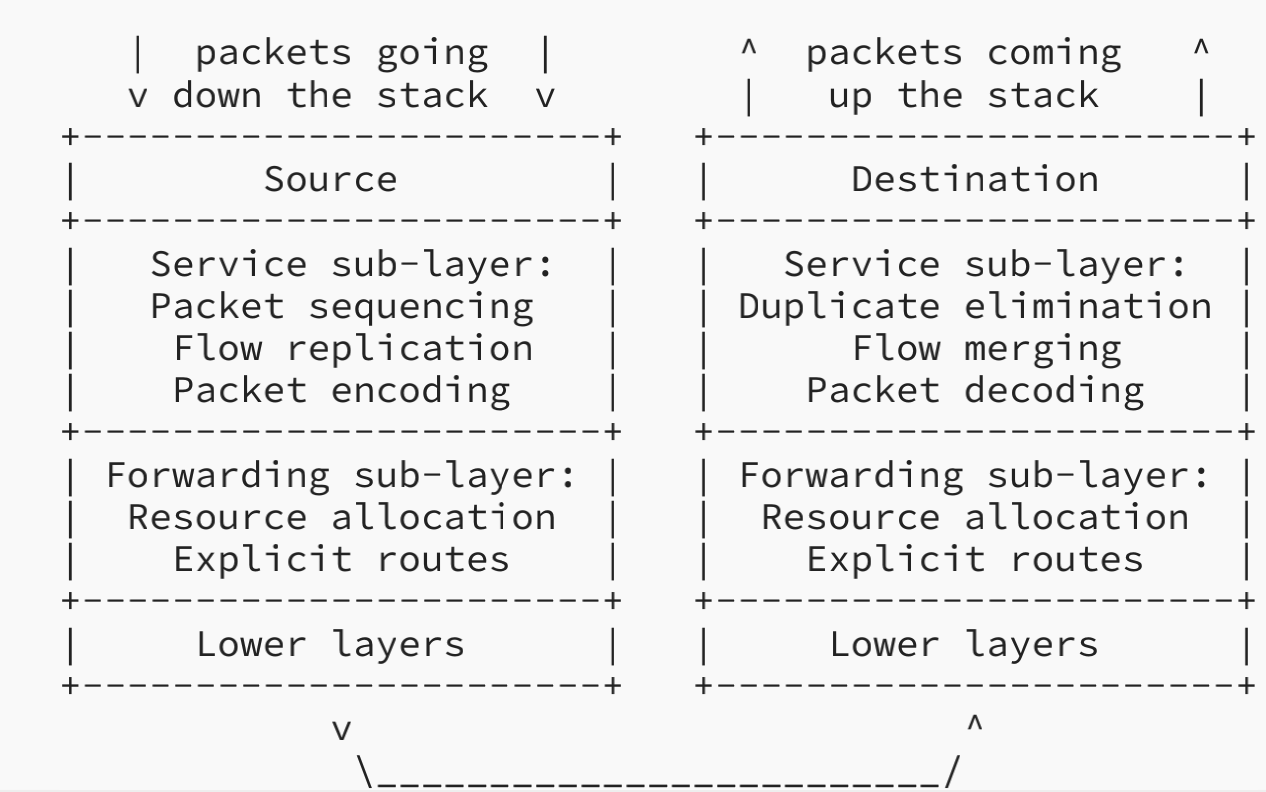
\includegraphics[width = 0.7\textwidth ]{Figures/DetNet protocol stack.png}
    \caption{DetNet protocol stack}
    \label{fig:stack}
\end{figure}

On the other hand, an overview of the DetNet network is also provided as shown in Fig.~\ref{fig:network}. A DetNet-enabled network is composed of DetNet edge and relay nodes, respectively. The DetNet edge nodes and relay nodes are interconnected by DetNet transit node which only support forwarding function. All DetNet nodes are connected to sub-networks, e.g. MPLS-TE, TSN, etc. 
Fig.~\ref{fig:stack}. 
\begin{figure}
    \centering
    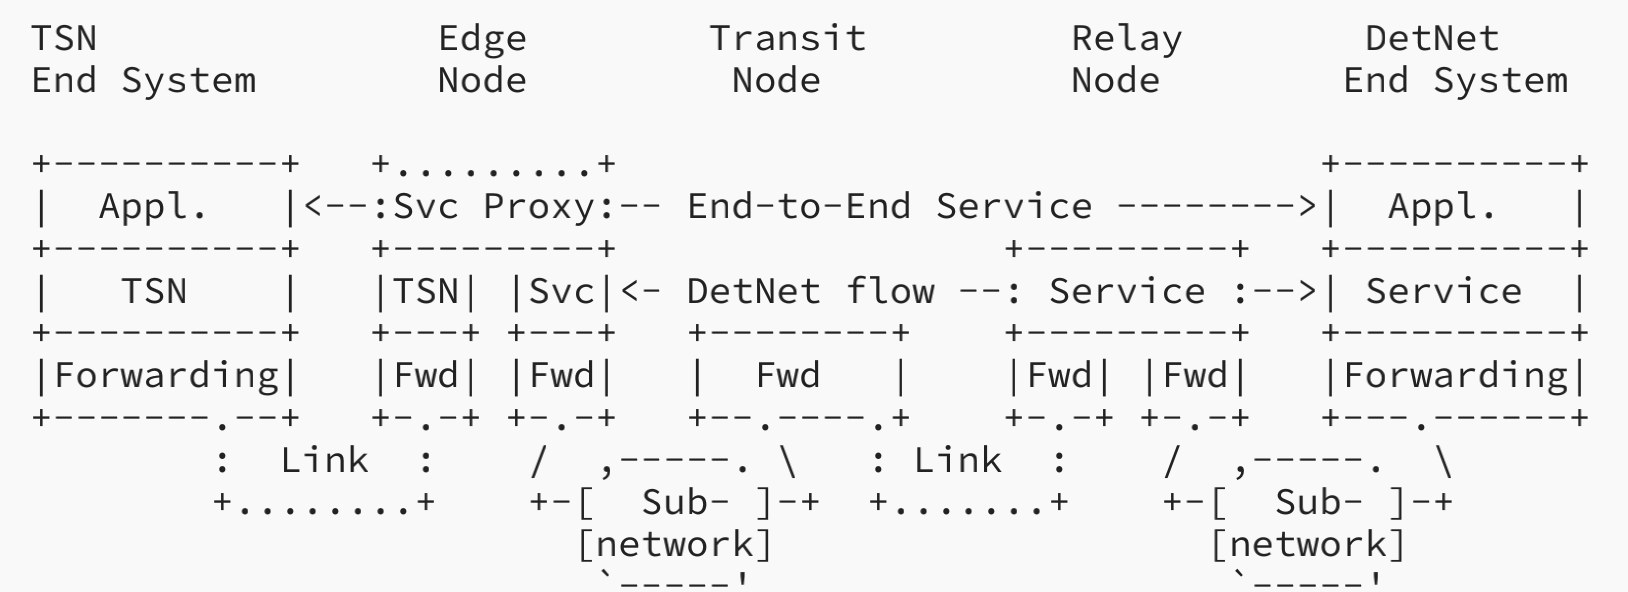
\includegraphics[width = 0.7\textwidth ]{Figures/DetNet overview.png}
    \caption{DetNet-enabled network}
    \label{fig:network}
\end{figure}
DetNet end systems are also categorized into fours classes in terms of forwarding sub-layer and service sub-layer awareness. It is worth noticing that if more DetNet unaware nodes are deployed as transit nodes, the DetNet QoS can be harmed due to lack of service protection and resource allocation for DetNet flows.

\begin{remark}
This RFC document gives a conceptual architecture of DetNet including fundamental techniques such as service protection, resource allocation, and explicit route. From my point of view, traffic classification and flow characterization is the base of realizing DetNet service. Packet duplication and elimination function placement and decision making is an interesting research topic. Since DetNet assumes a centralized controlled protocol, resource allocation is only feasible within small-scaled network with limited number of traffic flows. Network dynamics can be harmful to centralized-based method too. 
\end{remark}


\subsection{RFC 8678: Deterministic Networking Use Cases~\cite{grossman2019deterministic}}
This RFC identifies a range of applications and scenarios that requires deterministic services, i.e., guaranteed bandwidth, latency, etc. The use cases covers a large scope, including, professional audio and video (ProAV), electrical utilities, wireless for industrial applications, cellular radio, industrial machine to machine (M2M), private blockchain, network slicing, etc. Since so many topics are covered, part of them is summarised and analyzed here according to my personal interest. 

\subsubsection{Professional Audio and Video}
ProAV industries such cinema, music and film creation, live shows are transitioning from point to point single link per signal to packet based infrastructures to reduce cost and integrate with current IT infrastructures. Some key use cases in ProAV includes:
\begin{itemize}
    \item Uninterrupted streaming playback. Retransmission of ProAV for live playbacks is impractical as it is more time critical unlike file transfers. Buffering to provide delay space for retries alone is insufficient in time critical scenarios. FEC can be an option to address this issue.
    \item Synchronized streaming playback. Synchronization in this context mainly refers to the consistence between audio and video when multiple paths are taken for transmission. Typical tolerance for audio/video synchronization is one National Television System Committee (NTSC) video frame (about 33 ms). Current solution is to has the sink application delay all packets but on the slowest path. 
    \item Sound reinforcement. Sound reinforcement requires a maximum delay of 15~ms in total (from microphone to speaker). In some cases, such as beam-forming using multiple speakers, the latency should be within tens of microseconds.
    \item Secure transmission. Secure in this context refers to securely transmit sensitive traffics (such as amplifier control signals) to prevent harm to audience.
\end{itemize}
The future ProAV is anticipated to have the following features.
\begin{itemize}
    \item Interconnect L2 islands.
    \item High reliability streaming paths.
    \item Integration of reserved streams into IT networks.
    \item Sharing bandwidth with best-effort traffics to improve bandwidth efficiency. 
    \item Traffic Segregation. Prevent unnecessary process at devices with low cpu power.
    \item Multicast addressing to keep bandwidth utilization
   of shared links to a minimum. To ensure the multicast address is only associated to one stream.
   \item Reduced device costs due to reduced buffer memory.
\end{itemize}

\begin{remark}
RFC DetNet Architecture is capable of addressing several issues in ProAV. For example, packet duplication and elimination to provide high reliability streaming paths, explicit path and resource allocation to provide Diffserv services. Multicast addressing may require other function blocks to support.
\end{remark}


\subsubsection{Building automation system (BAS)}
The BAS is an essential component in IoT scenario which manages equipment and sensors in a building to improve living comfort. Key functions in BAS include monitor devices, store measured data, data analysis (e.g., fault detection), and control devices. Current BAS architecture contains two layers of network, namely management network, and field network. Management network is normally IP-based best-effort network, whereas field network is non-IP-based time-critical network. 

Future BAS anticipates lower energy consumption but  finer-grained environment monitoring with more sensors. Building networks will be connected to other networks, such as, enterprise network, the Internet, etc.  

\subsubsection{Wireless for industrial application}
Wireless networks are essential to industrial application in many aspect. Normally large amount of devices are involved in the network, where a small cost reduction may bring huge benefits.
Some existing wireless networks support deterministic QoS such
as 6TiSCH, but are not compatible with each other or IP traffic. Some common features include, precise scheduling, remote monitoring and scheduling management by path computation entity (PCE) and network management entity (NME). 

In the future, wireless networks are expected to enable converged transport of deterministic and best-effort traffic flows between real-time industrial devices and WANs via IP routing. 6TiSCH in particular can be co-developed with DetNet in terms of retries, schedule management, path management, IP interface, and security, etc.

\subsubsection{Cellular Radio}
The cellular network architecture includes ``Fronthaul", `` Midhaul", and ``Backhaul" network segments.  The fronthaul is the network connecting base stations to the Remote Radio Heads (RRHs) or antennas. The midhaul is the network that interconnects base stations (or small-cell sites).  The "Backhaul" is the network or links connecting the radio base station sites to the network    controller/gateway sites (i.e., the core of the 3GPP cellular network). 
Here how DetNet can help fronthaul to reduce delay is mainly discussed.

Current fronthaul networks typically consist of (1) Dedicated point-to-point fiber connection. (2) Proprietary protocols and framing. The midhaul and backhaul adopts IP-network or MPLS-TP, Clock distribution and synchronization using IEEE 1588 and syncE. 

The transport time budget covers scheduling/queueing delay, transmission delay, and link propagation delay. DetNet helps improve fronthaul network by controlling and reducing the delay budget consumption through precise resource allocation. For example,  control the bandwidth assignment of the fronthaul link and the scheduling of fronthaul packets over this link, provide adequate buffer
provisioning for each flow to reduce the packet loss rate.  
Apart from reducing delay, DetNet can provide flow isolation, e.g., flows from different network slices. 

Transport is also assumed to be error-free. The transport errors in fronthaul and midhaul refer to packet loss due BER, congestion, or network failure. Existing methods to eliminate traffic loss face serious challenges. For example, Retransmission and applying FEC introduce too much delay, redundant streams occupies high bandwidth.  In addition, the fronthaul links are assumed to be symmetric, i.e., with equal priority and cannot preempt or delay one another.

The future cellular radio networks are envisioned to be based on a mix of Xhauls. Some requests to achieve new cellular radio networks include: (1) Unified among all Xhauls. (2) Deployed in a highly deterministic network environment. (3) Capable of supporting multiple functional splits simultaneously. (4) Capable of supporting network slicing and multi-tenancy. (5) Capable of transporting both in-band and out-of-band control traffic. (6) Deployable over multiple data-link technologies.

\subsubsection{Network slicing}
Network slicing divides the underlying network infrastructure into several independent logical networks which share the same resources. Network slicing provides flexibility of resource allocation and service quality customization. 

DetNet can help improve network slicing from two perspectives. 
\begin{itemize}
    \item Across slices. DetNet should provide hard isolation among slices, i.e., different user's deterministic performance. 
    \item Within a slice.  Deterministic performance can be provided to both DetNet-aware slices and non-DetNet-aware slices.
\end{itemize}

A typical use case of DetNet in 5G is the hard service isolation bearer network. With DetNet, services of different slices would not compete for resources (e.g., bandwidth, reliability requirements) which lead to failure in QoS-guarantee. 

There are some limitations of DetNet in network slicing, too. For example, network slicing essentially requires multipoint-to-multipoint guarantees while DetNet provides point-to-point or point-to-multipoint. Scalability is another issue in centralized DetNet. (\textbf{Remark}: A distributed DetNet solution is essential in addressing this issue.)

\begin{remark}
In this RFC document, a variety of potential DetNet use cases ($9$ in total) are introduced. The analysis of each use case follows the sequence: (1) Mechanism overview. (2) Existing solutions/research status. (3) Feasibility of DetNet usage. (4) Request to DetNet.

The common requests of the use cases can be summarised as follows.
\begin{itemize}
    \item Strict latency-guaranteed service. End-to-end delay-guarantee is the essential feature of DetNet. Both delay upper bound and lower bound should be guaranteed. Apart from that, a tight jitter is also desired in some time-critical applications such as ProAV.  
    \item Hard service isolation. Service isolation ensures QoS-guarantee among multiple traffics as well as easier management, allows more flexibility. 
    \item Coexistence with best-effort traffics. Adoption of DetNet should be practically feasible. DetNet traffics should not affect best-effort traffics while the reserved resources should be available to the best-effort whenever possible.
\end{itemize}

\end{remark}


\section{Deterministic networking solutions}
In this section, the note summarizes some existing solutions to guarantee one or more aspects of quality-of-service (QoS), for example, end-to-end delay, jitter, reliability, throughput, etc. These solutions may not incorporate the IETF DetNet architecture, but provide a way of guaranteeing performances. Since there is no existing standards to support deterministic networks, most solutions are proposed based on certain assumptions which may be addressed at different layers, e.g., time synchronization, packet tags that can be carried by packets for routing/scheduling purposes, precise flow characterization, etc. Therefore, the feasibility and efficiency of the solutions will be discussed in the remarks, too.

\subsection{Towards Large-Scale Deterministic IP Networks~\cite{liu2021towards} -- 2021}

This paper proposed a scalable large-scale deterministic network (LDN) architecture to provide end-to-end delay-guaranteed service and bounded jitter in IP networks.  The LDN architecture decouples the network into data plane and control plane as shown in Fig.~\ref{fig:LDN}. The LDN routers in the data plane adopts a traffic shaping mechanism at the ingress-gateway which prevents network congestion caused by bursty traffics, and a cyclic queue mechanism at each LDN router which forward packets in a round-robin fashion to reduce jitter and delay. In the control plane, LDN considers a centralized controller that computes the traffic shaping parameter as well as the routing decision at each hop. In addition, LDN enables DiffeServ by sharing the bandwidth between time-critical traffics and best-effort traffics.
\begin{figure}
    \centering
    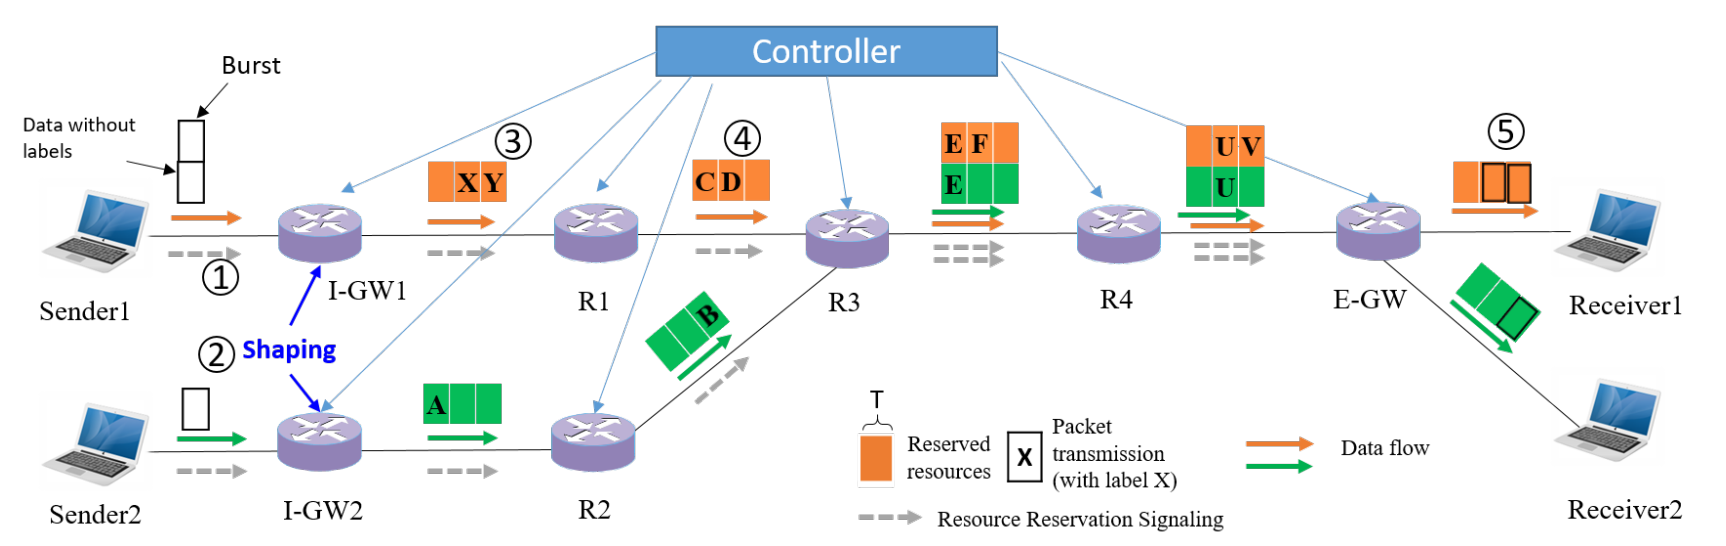
\includegraphics[width = \columnwidth]{Figures/LDN.png}
    \caption{LDN architecture}
    \label{fig:LDN}
\end{figure}

The cyclic queue forwarding (CQF) has been proved effective in bounding latency and jitter. LDN adopts the similar idea, where $3$ queues are considered. At the traffic shaping mechanism, bursts are spread over $n$ cycles at the cost of introducing a shaping delay of $nT$. At the cyclic scheduling mechanism, three queues at each port takes in and forward packets in sequence. Only one queue forwards packet per cycle while the rest absorbs the arriving packets. This scheduling policy allows a worst e2e delay of $D_{worst} = T + \sum_{i=2}^h (\tau_i + T)$ and a minimum e2e delay of $D_{min} =  \tau_h + \sum_{i=2}^{h-1} (\tau_i + T)$, where $h$ is the number of hops in a given path, $T$ is the time of a cycle, $\tau_i$ is the gap between cycles of different nodes. 
An essential part of LDN, however, is not explained in the paper. Upon receiving the packets from the upstream nodes, the core routers in LDN determine their output labels (cycle or queue)  according to their carrying label independent of flows. This mapping process is the key to guarantee e2e delay. The mapping between two nodes depends on the propagation and transmission delay, thus, a dynamic detection and re-learning the mapping relationship mechanism is required. However, this part is not explained. 

The centralized controller computes the shaping parameter and routing path for each flow to maximize the overall accepted traffics. The solution to the optimization problem yields the proposed CGRR routing algorithm. A proof-of-concept (PoC) prototype of LDN is implemented. The results show that LDN is capable of bounding the jitter within $2T$. The scalability of LDN is verified via simulations on OMNet++ using a real ISP
topology (AS 1239 of Sprint). 

\begin{remark}
LDN provides a feasible solution to delay-guaranteed service with bounded jitter. However, the drawbacks of LDN are also obvious. Firstly, LDN requires a guaranteed or predictable propagation and transmission delay between two routers to ensure the packets enters the right cycles of the next-hop. Since the gap between two cycles can be very small (at the levels of microseconds), link state variation can impose great impact to LDN. Secondly, the dynamic link state detection and mapping mechanism can be hard to implement in practice due to the dynamic features of network. Thirdly, the centralized structure is vulnerable to topology variations. Apart from the computation complexity at the controller, the controller needs to run CGRR every time the network topology changes including the change of traffic flows which may impose higher cost and delay.

\end{remark}



\subsection{Optimization of Flow Allocation in Asynchronous Deterministic 5G Transport Networks by Leveraging Data Analytics~\cite{prados2021optimization} -- 2021}

This paper targeted on addressing the flow allocation problem in 5G backhaul networks (BN) realized as asynchronous time-sensitive network (TSN). The proposed solution named Next Generation Transport Network Optimizer (NEPTUNO) works based on asynchronous traffic shapper (ATS) which is a key component in TSN networks.  NEPTUNO leverages data analytic to solve the flow allocation problem. NEPTUNO is essentially an offline method that computes the long-term configurations for the whole network considering different types of traffics. Thus, the allocation schemes are predetermined, and the access control mechanism (ACM) becomes lightweight. In addition to NEPTUNO, an online approach is also proposed in this paper. The online approach computes the allocation configuration upon each arrival of flow. 

\begin{figure}
    \centering
    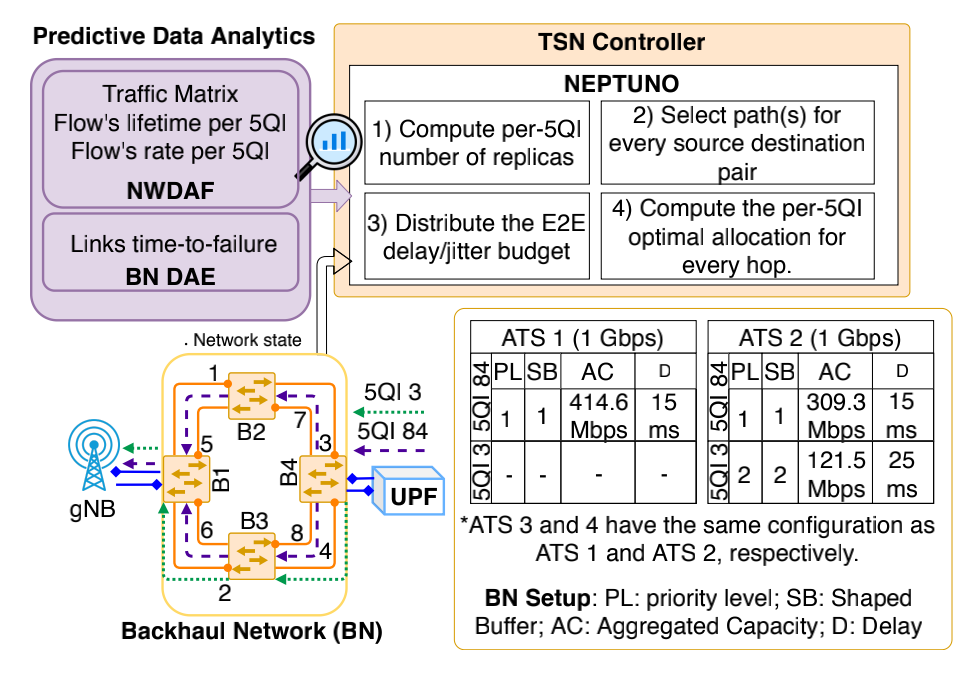
\includegraphics[width=.6\columnwidth]{Figures/NEPTUNO.png}
    \caption{System model of NEPTUNO}
    \label{fig:NEPTUNO}
\end{figure}

The goal of NEPTUNO is to minimize flow rejection ratio while guaranteeing QoS performance. To achieve this, the paper formulated the scheduling problem by setting the QoS performance metrics as constraints, and the reject ratio-related parameters as minimization objective. More specifically, NEPTUNO considers three key QoS metrics, namely the e2d delay, jitter, and reliability. The upper bound of each metrics are derived based on the assumption that ATS at each node is applied. By solving the flow allocation problem, NEPTUNO goes through the following subproblems in sequence: i) Compute the number of packet replicas to ensure the reliability requirement. Note that each replica takes different and disjoint path. ii) Run the path selection algorithm to achieve load balancing.  iii) Distribute the delay/jitter budget along the paths previously determined based on link capacity. iv) Computes the optimal configuration for each last hop by solving the Mixed Integer Linear Program (MILP). Specifically, it finds the 5QI-to-shapped buffers and 5QI-to-priority assignments, and the per-5QI maximum aggregated capacity to be allocated at the corresponding ATS. It is worth noticing that NEPTUNO distinguishes two types of ATS in terms of location, i.e., transit hops and last hops. The optimization objective at the transit hops focusing on controlling the number of flows to the target number, while the last hop ones aims at minimizing the rejection ratio. 

As for the online approach, it is essentially a simplified version of NEPTUNO. Firstly, it computes the number of disjoint paths to ensure the reliability requirement. Then the optimal paths that achieves load balance are selected. Then for every ATS along the path, the MILP at each ATS is solved to give the flow allocation scheme. 

The simulation results show that NEPTUNO provides a rejection ratio of $10\% - 20\%$ higher than the optimal values but achieves much lower time and computation cost as the number of links increases. 
The online approach achieves a similar performance as NEPTUNO in minimizing rejection ratio with various 5G QoS identifiers(5QI).

\begin{remark}
The paper mainly targets on the flow allocation problem in 5G backhaul networks based on the application of the ATS module. The proposed NEPTUNO is essentially a centralized solution since it requires the knowledge of network topology and link occupancy of paths. NEPTUNO shines light on the application of data analytics in solving network flow allocation problems. This provides us with a new idea for simplifying optimization problems in networking.
\end{remark}


\subsection{Delay-Guaranteed Cross-Layer Scheduling in Multihop Wireless Networks~\cite{xue2012delay} -- 2013}
In this paper, the author proposed a cross layer scheduling algorithm incorporating congestion control in the transport layer and scheduling of flow in the link layer. The paper aimed at guaranteeing QoS requirement such as throughput, end-to-end delay, and data rate, while stablizing the queue backlogs. Three types of virtual queues are designed to achieve the goals. Different from previous works based on the popular back-pressure algorithm, where the throughput optimality is achieved (proved) at the cost of large queue backlog, the virtual queues constructed in this paper are responsible for guaranteeing the QoS requirements. It is worth mentioning that the paper assumes a finite buffer size unlike previous studies where an infinite buffer size is assumed.
The proposed algorithm achieves an $\epsilon$-close-to-optimal in throughput with a tradeoff of $O(\frac{1}{\epsilon})$ in guaranteeing average delay. 

\begin{figure}
    \centering
    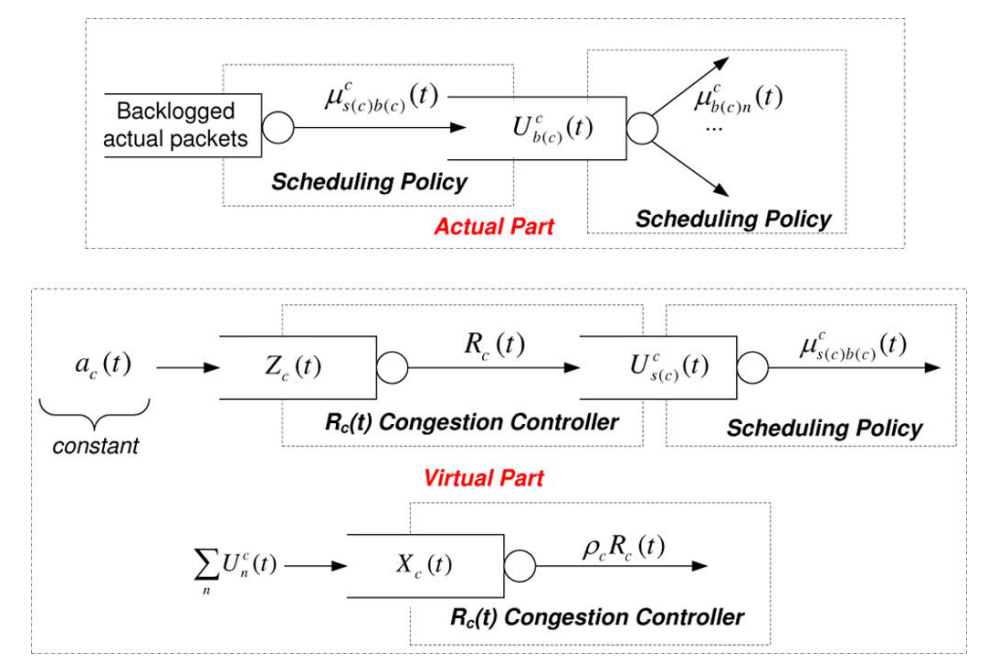
\includegraphics[width = 0.7\columnwidth]{Figures/CorssLayer.png}
    \caption{Virtual queues of a source node in Cross-Layer scheduling}
    \label{fig:crossLayer}
\end{figure}

$U^c_n(t)$ denote the backlog of flow $c$ waiting for transmission at node $n$, $U^c_s(t)$ denote the virtual queue at the transport layer, $Z_c(t)$ the virtual service queue, and $X_c(t)$ the virtual delay queue. $U_s(t)$ and $Z_c(t)$ is non-zero only at the source node, and there is no backlog at the sink node, i.e., $U^c_n(t) = 0 ~ \forall t$.  A congestion controller model based on the virtual queues is formulated, where the input rate is dependent on a control variable $R_c(t)$. The joint scheduling is modeled based on the Max-Weight problem, where the average delay and minimum data rate are set as the constraints. The solution to the Max-Weight problem yields the scheduling policy. The policy is proved to stabilize the virtual queues, and achieve an $\epsilon$-close-to-optimal in throughput with a tradeoff of $O(\frac{1}{\epsilon})$ in guaranteeing average delay. 

In addition, the paper considered a more practical scenario, where the feedback delay is considered. The delayed feedback is caused by obtaining the queue backlog information from the network. The model is modified based on a local queue backlog estimation, but can be further extended to a distributed algorithm. The distributed algorithm still achieves an average end-to-end delay of order $O(\frac{1}{\epsilon})$. Since the original Max-Weight problem is NP-hard, the paper reduced the proposed algorithm to a suboptimal one with the reduced factor of $\gamma \in (0,1)$. The suboptimal algorithm is also proved to achieve guaranteed minimum data rate, end-to-end delay, and a throughput $\epsilon$-close to the $\gamma$ fraction of the optimal throughput. 

\begin{remark}
This paper is theoretically solid with sufficient proofs and derivation. The overall logic is clear that the proposed network scheduling framework containing three virtual queues can achieve $O(\epsilon)$ throughput optimality while guaranteeing end-to-end delay ($O(\frac{1}{\epsilon})$) and minimum data rate. The approach however, only theoretically analyzed the feasibility of guaranteeing the time average end-to-end delay. A hard delay-guaranteed at the real-time level solution is required in Deterministic Network.
\end{remark}

\subsection{Optimal Control of Wireless Networks with Finite Buffers~\cite{le2010optimal} -- 2010}
This paper considers the network optimization problem for wireless networks with finite buffers. The proposed algorithm considered two scenarios depending on whether the traffic arrival rate is inside or outside the capacity region. The algorithm jointly optimizes flow control, routing, and scheduling to achieve high network utility and bounded queue backlog. Similar to other works, a discrete time-based network model is constructed. In their system model, only the buffer size of the internal nodes (internal buffer) is assumed to be finite while that of the source node (ingress buffer) is assumed to be infinite. In addition, the corresponding queue length of the destination node is always empty. The paper first discussed that the network is always stable due to the finite buffer size. Then a network utility maximization problem is formulated based on a $\epsilon$-stripped throughput region. The algorithm that solves the maximization problem yields the flow control and routing/scheduling control, respectively. The algorithm has been proved that give an $\epsilon >0$, the utility and ingress queue backlog can be bounded if the internal buffer size satisfy $l_c > \frac{N-1}{2\epsilon}$, where $N$ is the number of nodes in the network. 

Some numerical results are presented to show verify the performance of the proposed algorithm. The proposed algorithm achieves significant reduction in ingress buffer backlog and internal buffer backlog compared with the CLC2b algorithm where an infinite buffer size is assumed. 

\begin{remark}
The paper proved that the proposed algorithm can provide a lower bound for network utility and an upper bound for ingress queue length given a finite internal buffer size. This is very useful to our DSR work. However, the paper failed to consider the delayed feedback of ingress queue information (IQI) as well as obtaining next-hop queue length in the routing/scheduling algorithm, which also need to be considered in our work.
\end{remark}





\section{Appendix A}


\bibliographystyle{IEEEtran}
\bibliography{References}
\end{document}